\pdfoutput=1

\documentclass[11pt,DIV=16,parskip=half]{scrartcl}
\usepackage{algorithm,algorithmic}
\usepackage{amsmath,amssymb,amsfonts}
\usepackage{graphicx}
\usepackage{hyperref}
\usepackage{multirow}
\usepackage{svg}
\usepackage{textcomp}
\usepackage[svgnames]{xcolor}
\usepackage{tikz}
\usetikzlibrary{shapes.geometric, positioning, arrows, arrows.meta, decorations, decorations.pathmorphing, backgrounds, fit, petri, chains}

\tikzset{
	component/.style={
		font=\small\itshape,
text width = 2cm},
	group/.style={
		draw=gray!40,
		dashed,
		decoration={zigzag,
		amplitude=0.5}
	},
	outline/.style={
		draw=black!50,
		inner sep=5pt,
		decorate,
		decoration={random steps,
		segment length=10pt,
		amplitude=1pt}
	},
	wip/.style={
		minimum height=1cm,
		minimum width= 2cm,
		dashed,
		rounded corners=2pt,
		draw=gray!80,
		fill=LightCoral!30
	},
	existing/.style={
		minimum height=1cm,
		minimum width= 2cm,
		rounded corners=2pt,
		draw=gray!80,
		fill=gray!20
	},
	flowWip/.style={
		draw=gray!80,
		dashed,
		-Stealth},
	flowExisting/.style={
		draw=gray!80,
		-Stealth
	},
}


\usepackage[backend=biber, bibencoding=utf8, giveninits=true,
maxbibnames=99, % show all authors in the bibliography
maxalphanames=1, minalphanames=1, style=ieee, backref=false]{biblatex}
% Sets the bib file
\addbibresource{refs.bib}

% Basic information
\title{Temporal Logic in a Multi-Level Abstraction Hardware Compiler}
\author{Tobias Wölfel, \href{mailto:tobias.woelfel@hm.edu}{tobias.woelfel@hm.edu}}
\date{May 2025}

%TODO add acronyms

\begin{document}
\maketitle

\section{Introduction}
% Limit: 150 words
% Actual: 299 words

Hardware designs are getting more complex and diverse as fabrication technology
evolves and specialized solutions offer a competitive advantage.
This complexity must be handled by the design tools as well as the verification
flow.
Due to the increasing complexity and the associated costs, a correct design is
critical.
With that, design verification is crucial and also ubiquitous, making it a
critical component in the hardware design process.

% TODO: add picture with signal sequence
One way to ensure correct behaviour is to specify a desired signal sequence and
following a match, check for a give state of the design.
A linear sequence of events can be expressed with concurrent SystemVerilog
Assertions, which are fundamentally based on linear temporal logic (LTL).
Concurrent SystemVerilog Assertions are widely supported in proprietary
industry tools, but only marginally in the open-source semiconductor ecosystem.
% not really true, they can also use proprietary tools
The missing support hinders verification capabilities in the open-source
hardware design field, which is becoming more prominent in academic research.
Additionally, it prevents research in the area of temporal logic for
verification, analysis and optimization for hardware designs.

A project which offers a framework for hardware designs and basic support for
SystemVerilog is Circuit IR Compilers and Tools (CIRCT).
CIRCT builds on top of Multi-Level Intermediate Representation (MLIR) and
allows to have different levels of abstraction of the design at the same time.
An advantage of CIRCT's design is the modularity based on a variety of dialects
and transformation passes, which allows for different input and output formats.

In this work, CIRCT will be extended to support linear temporal logic for
multiple input formats.
In order to make use of the verification for consuming tools, different
transformation methods will be investigated.
Research will focus on representation formats and abstractions for temporal
logic, with the goal of leveraging this verification information to improve the
integrated circuit design process itself.

\section{Related Work}
% related work and state of the art
% Overview of relevant approaches and detailing most similar solutions

% Limit: 300 words

% - LTL support in Chisel, higher abstraction, greater need to verify the lower levels
% - SystemVerilog Assertions and support in open source tools
% - What can be done with LTL?

\begin{itemize}
  \item LTL and SVA in open source tools
  \item assertions in simulation, FPGAs
  \item LTL formula to automata transformation (state machines to create matches and checks)
  \item analysis and optimization with LTL properties?
  \item power, active region analysis in industry by benchmarking, running code? static analysis available?
\end{itemize}

\section{Thesis Objective}
% Based on the related work, show the research gap addressed in the thesis
% Research questions the thesis will answer
% Describe the overall expected outcome of your research.

% Limit: 150 words
% Actual: 180 words

% TODO Reformulate this
The support of linear temporal logic as a method, and SystemVerilog Assertions
in general is only partially available in open-source hardware design tools.
With this comes a lack of transformation to analogous representations which can
be consumed by other tools.
As there is also no available environment in which a hardware design is
represented in conjunction with the temporal properties, no research is
possible in the area of hardware design analysis and optimization based on
signal sequences.

This thesis focuses on the benefits of temporal logic for hardware designs in
open-source design tools.

To achieve this goal, the following main research questions must be addressed:

\begin{itemize}
  \item How can linear temporal logic be represented in a multi-level
    intermediate representation?
  \item How must transformation methods be designed in order to propagate the
    user-specified verifications to later stages in the tool flow?
  \item Which insights can be gained from the specified properties and
    sequences?
\end{itemize}

With this thesis, a basis for more capable verification of hardware designs
will be created, as well as a first look into ways to make further use of
verification specifications.

\section{Research Outline}
% Sketch outline
% Problems faced, planned solutions?
% External requirements, how to meet them?
% Progress measurement, success criteria?
% Argument for getting Dr.-Ing.

% Figures, schemes, tables or itemized formatting

% Limit: 500 words
% Actual: 423 words

The research will be structured into two topics.
The first part will lead to a suitable representation of the temporal
descriptions as a dialect in CIRCT, while the second part will focus on making
use of the new representations to find improvements for the hardware design.

In order to consume the SystemVerilog Assertions, the SystemVerilog support of
CIRCT must be extended.
The lexing, parsing and a first elaboration of the SystemVerilog description is
handled by Slang, a separate project, which comes with a high language feature
completeness for SystemVerilog, while providing programmatic methods to extract
information from the generated Abstract Syntax Tree (AST).
With the design represented in the AST, a translation into CIRCT's dialects
follows.
A suitable representation and dialect translation path for SVAs must be found.
A subset of SVAs may be selected to be supported in the first step, in order to
ensure progress.
% state explosion possible?
Dialect transformations, if possible and realizable, for different output
variants will provide new benefits for later stage tools.
The transformations might require additional dialects in order to represent
different forms of matching sequences and condition verifiers.
In this stage, research will focus on finding an optimal representation of the
temporal logic.

With the new dialect available, research will shift to utilize the added
information.
One possibility of extracting new insights lies in the analysis of the logic
elements described by the temporal properties.
For this a relation between the verification and the design has to be found,
together with a way of annotating the findings as well as how this can be used
by other tools.
Another possibility may be in design optimization.
Again, based on the temporal properties, which provide additional information
for the signals, an optimization might be possible on the utilized cells and
the connections between them.
The optimization might be possible at different levels of abstraction of the hardware.
Combining the optimization with the temporal logic dialect will provide
feedback on the suitability of the representation formulated in the first part
of the research project.

The research merits a Dr.-Ing. degree through two contributions to electronic
design automation for integrated circuits.
First, it advances verification methodology in hardware design by extending a
multi-level hardware representation with an abstracted temporal logic
representation, while building an improved framework for verification in the
open-source hardware ecosystem, enabling a higher correctness of hardware
designs.
Second, the research explores how verification specification of temporal logic
can be utilized in the design process, in contrast to only forwarding it to
tools later in the design flow, gaining additional insights into the design.

\begin{figure}[htb]
\centering
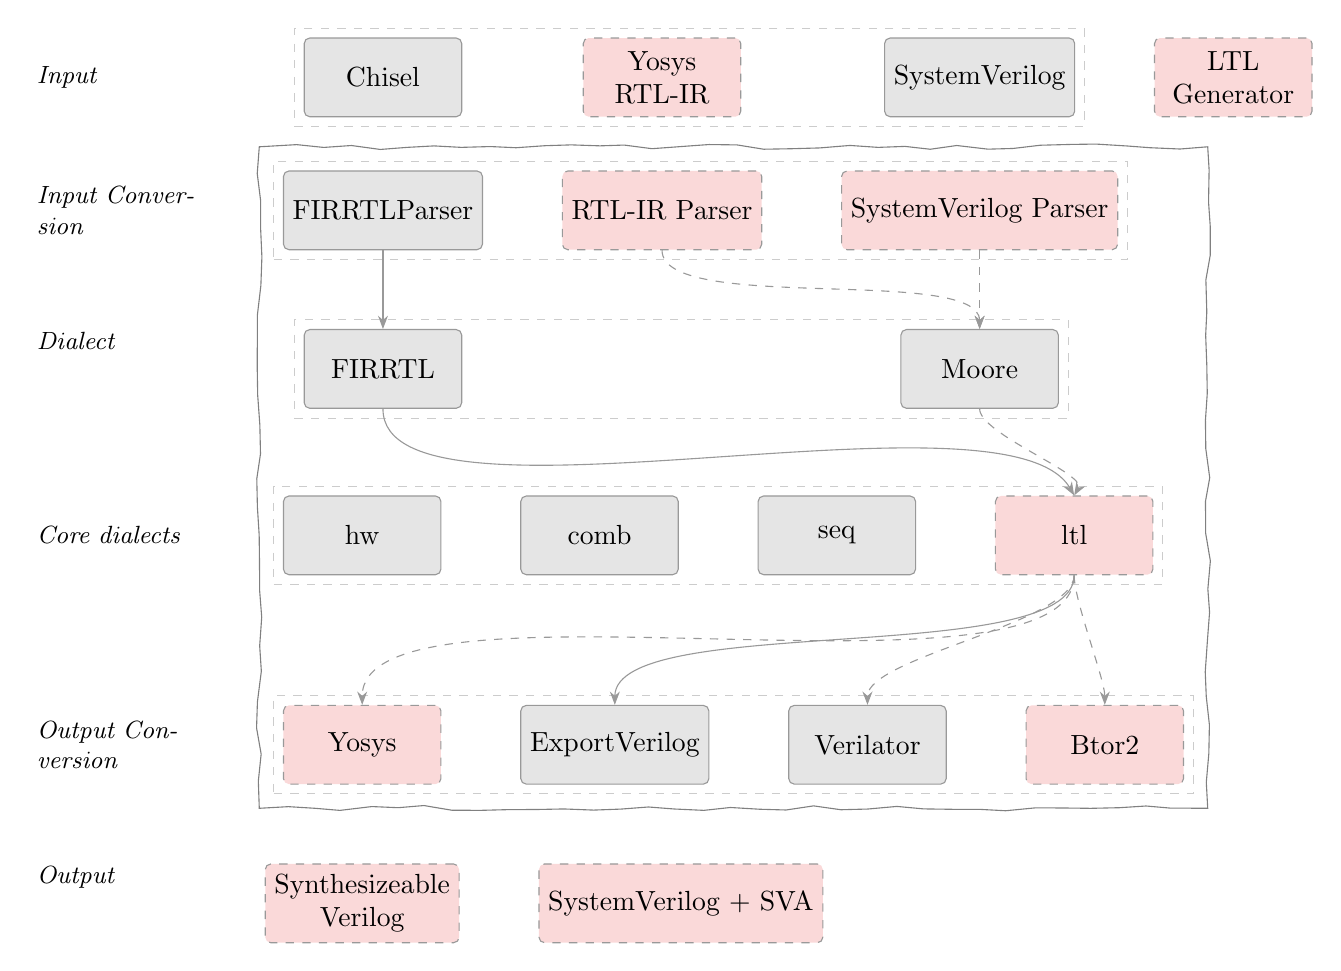
\begin{tikzpicture}
	% input languages
	\node [component] (inputLanguages) {Input};
	% input conversion
	\node [component, below=of inputLanguages] (inputConversion) {Input Conversion};
	\node [existing, right=of inputConversion] (firrtlParser) {FIRRTLParser};
	\node [wip, right=of firrtlParser] (yosysParser) {RTL-IR Parser};
	\node [wip, right=of yosysParser] (slang) {SystemVerilog Parser};
	\node [group, fit=(firrtlParser) (yosysParser) (slang)] (inputConversionBbox) {};

	% input languages (cont. with alignment to input conversion)
	\node [existing] at (firrtlParser|-inputLanguages) (chisel) {Chisel};
	\node [wip, align=center] at (yosysParser|-inputLanguages) (yosysrtl) {Yosys\\RTL-IR};
	\node [existing] at (slang|-inputLanguages) (sv) {SystemVerilog};
	\node [wip, right=of sv, align=center] (ltlgen) {LTL\\Generator};
	\node [group, fit=(yosysrtl) (sv) (chisel) (yosysrtl) (sv)] (inputR) {};

	% Dialects
	\node [component,below=of inputConversion] (dialects) {Dialect};
	\node [existing, below=of firrtlParser] (firrtl) {FIRRTL};
	\node [existing, below=of slang] (moore) {Moore};
	\node [group, fit=(firrtl) (moore)] (dialectsR) {};

	% core dialects
	\node [component,below=2cm of dialects] (coreText) {Core dialects};
	\node [existing, right=of coreText] (hw) {hw};
	\node [existing, right=of hw] (comb) {comb};
	\node [existing, right=of comb] (seq) {seq};
	\node [wip, right=of seq] (ltl) {ltl};
	\node [group, fit=(hw) (comb) (seq) (ltl)] (coreR) {};

	% output conversion
	\node [component,below=2cm of coreText] (outputConversion) {Output Conversion};
	\node [wip, right=of outputConversion] (yosys) {Yosys};
	\node [existing, right=of yosys] (exportVerilog) {ExportVerilog};
	\node [existing, right=of exportVerilog] (verilator) {Verilator};
	\node [wip, right=of verilator] (btor2) {Btor2};
	\node [group, fit=(yosys) (exportVerilog) (verilator) (btor2)] (outputConversionBbox) {};

	% CIRCT
	\node [outline, fit=(inputConversionBbox) (coreR) (outputConversionBbox)] (circt) {};

	% Output Language
	\node [component, below=of outputConversion] (outputLanguages) {Output};
	\node [wip, below=of yosys, align=center] (verilog) {Synthesizeable\\ Verilog};
	\node [wip, right=of verilog, align=center] (verilog) {SystemVerilog + SVA};

	% Connect input conversion to dialects
	\draw [flowWip] (yosysParser.south) to [out=-90, in=90, looseness=0.5] (moore.north);
	\draw [flowWip] (slang) -- (moore.north);
	\draw [flowExisting] (firrtlParser) -- (firrtl);

	% Connect dialects to core
	\draw [flowExisting] (firrtl.south) to [out=-90, in=120, looseness=0.5] (ltl.north);
	\draw [flowWip] (moore.south) to [out=-90, in=60, looseness=0.5] (ltl.north);

	% Ltl to all output conversions
	\draw [flowWip] (ltl) to [out=-90, in=90, looseness=0.5] (yosys);
	\draw [flowExisting] (ltl) to [out=-90, in=90, looseness=0.5] (exportVerilog);
	\draw [flowWip] (ltl) to [out=-90, in=90, looseness=0.5] (verilator);
	\draw [flowWip] (ltl) to [out=-90, in=90, looseness=0.5] (btor2);
\end{tikzpicture}
	\caption{LTL dialect as a central component in enabling verification support across a wide range of open source EDA tools.}
	\label{fig:toolOverview}
\end{figure}

\printbibliography

\end{document}
